% Phase 4 research paper -- IEEE journal template (IEEEtran).
% Compile on Overleaf (IEEEtran is built in) or any full TeX Live:
%   pdflatex main && bibtex main && pdflatex main && pdflatex main
% If IEEEtran.cls is missing, an IEEE-like fallback layout (ieeefallback.sty) is used instead.
\IfFileExists{IEEEtran.cls}
  {\documentclass[journal]{IEEEtran}}
  {\documentclass[10pt,twocolumn,letterpaper]{article}\usepackage{ieeefallback}}
\usepackage{cite}
\usepackage{amsmath,amssymb}
\usepackage{graphicx}
\usepackage{booktabs}
\usepackage{multirow}
\usepackage{array}
\usepackage{algorithm}
\usepackage{algpseudocode}
\usepackage{xcolor}
\usepackage{url}
\usepackage[hidelinks]{hyperref}
\graphicspath{{figures/}}
% generated by paper/gen_tables.py -- do not edit by hand
\newcommand{\RnTrain}{66,182}
\newcommand{\RnTest}{145,475}
\newcommand{\RnTestBen}{21,372}
\newcommand{\RnTestAtk}{124,103}
\newcommand{\RnTrainBen}{6,863}
\newcommand{\RattackShare}{85\%}
\newcommand{\RmainFone}{0.9987}
\newcommand{\RmainCIlo}{0.998}
\newcommand{\RmainCIhi}{0.999}
\newcommand{\RmainMCC}{0.997}
\newcommand{\RmainFPR}{0.42\%}
\newcommand{\RmainFNR}{0.006\%}
\newcommand{\RmainTTDmed}{50}
\newcommand{\RmainTTDmean}{49}
\newcommand{\RmainPone}{0.708}
\newcommand{\RmainExt}{0.631}
\newcommand{\RmainSize}{312}
\newcommand{\RmainLat}{0.58}
\newcommand{\RmainThr}{85,882}
\newcommand{\RmainDefer}{0.8\%}
\newcommand{\RmainPortMap}{99.9\%}
\newcommand{\RedgeFone}{0.9856}
\newcommand{\RedgeFPR}{4.75\%}
\newcommand{\RedgeSize}{4.6}
\newcommand{\RedgeLat}{0.55}
\newcommand{\RcloudFone}{0.9971}
\newcommand{\RdtFone}{0.9985}
\newcommand{\RdtFPR}{0.27\%}
\newcommand{\RdtPone}{0.791}
\newcommand{\RdtSize}{4.6}
\newcommand{\RdtLat}{0.57}
\newcommand{\RdtHolm}{0.32}
\newcommand{\RrfFone}{0.9957}
\newcommand{\RrfFPR}{1.32\%}
\newcommand{\RrfTTDmed}{60.0}
\newcommand{\RrfTTDend}{$<$0.01}
\newcommand{\RrfPone}{0.433}
\newcommand{\RrfSize}{657}
\newcommand{\RrfLat}{13.21}
\newcommand{\RrfThr}{39,131}
\newcommand{\RrfExt}{0.666}
\newcommand{\RlatRatio}{23}
\newcommand{\RttdRatio}{1,200}
\newcommand{\RifPone}{0.060}
\newcommand{\RhyFPR}{16.0\%}
\newcommand{\RbestPtwo}{0.8728}
\newcommand{\RbestPtwoName}{CNB}
\newcommand{\RimpAbs}{+0.1258}
\newcommand{\RimpRel}{+14.4\%}
\newcommand{\RknnFone}{0.7395}
\newcommand{\RknnSynRec}{0.3\%}
\newcommand{\RknnLagRec}{0.1\%}
\newcommand{\RknnLat}{2.62}
\newcommand{\RknnSize}{1,515}
\newcommand{\RknnSpeed}{4.5}
\newcommand{\RwinOne}{0.9989}
\newcommand{\RwinTwo}{0.9965}
\newcommand{\RwinThreeA}{49}
\newcommand{\RwinThreeB}{1.76}
\newcommand{\RhvN}{0.917}
\newcommand{\RhvR}{0.946}
\newcommand{\RhvG}{0.929}
\newcommand{\RfrontN}{55}
\newcommand{\Revals}{799}
\newcommand{\RfrontTrees}{49}
\newcommand{\RloaoMin}{99.9\%}
\newcommand{\RloaoTypes}{6}
\newcommand{\RextBest}{0.728}
\newcommand{\RextBestName}{GA (F1 only) best}
\newcommand{\RrevRF}{0.934}
\newcommand{\RrevMain}{0.597}
\newcommand{\RrevRFin}{0.972}
\newcommand{\RdirExt}{0.814}
\newcommand{\RdirFPR}{46\%}
\newcommand{\RtempExt}{0.280}
\newcommand{\RnoTempExt}{0.698}
\newcommand{\RabSTwoTTD}{97}
\newcommand{\RabSTwoLat}{6.65}
\newcommand{\RabSTwoF}{0.9984}
\newcommand{\RabSOneF}{0.9974}
\newcommand{\RabFullTTD}{49}
\newcommand{\RabFullLat}{0.63}
\newcommand{\RabNoneF}{0.9990}
\newcommand{\RabAllExt}{0.451}
\newcommand{\RabIntF}{0.9760}
\newcommand{\RabIntFPR}{7.9\%}
\newcommand{\RabTempExt}{0.753}
\newcommand{\RbalNM}{0.9051}
\newcommand{\RbalCW}{0.9984}
\newcommand{\Rspear}{0.69}
\newcommand{\RpilotSpear}{-0.28}
\newcommand{\RstressMain}{99.99\%}
\newcommand{\RstressRF}{97.9\%}
\newcommand{\Rmissed}{7}
\newcommand{\RdnsFP}{92\%}
\newcommand{\RpilotFone}{0.9892}
\newcommand{\RpilotSyn}{34.2\%}
\newcommand{\RpilotExt}{0.425}
\newcommand{\RmainSyn}{99.9\%}
\newcommand{\RpilotHvN}{0.955}
\newcommand{\RpilotHvR}{0.948}
\newcommand{\ReOneD}{5}
\newcommand{\ReNone}{3}
\newcommand{\ReTone}{50}
\newcommand{\ReNtwo}{4}
\newcommand{\ReTtwo}{100}
\newcommand{\ReFeat}{12}
\newcommand{\ReTlo}{0.032}
\newcommand{\ReThi}{0.680}
\newcommand{\RnDetectors}{20}

\newcommand{\fone}{\mathrm{F}_1}
\newcolumntype{L}[1]{>{\raggedright\arraybackslash}p{#1}}
\newcommand{\authornote}[1]{\textcolor{red}{[#1]}}

\begin{document}

\title{Early-Window Cascaded Detection of DDoS Attacks with Multi-Objective Accuracy--Time--Cost Optimisation}

\author{\IEEEauthorblockN{Dilawaiz Hameed and Mariam Shaiq}
\IEEEauthorblockA{FAST School of Computing, National University of Computer and Emerging Sciences (FAST-NUCES), Islamabad, Pakistan\\
Email: \{i232518, i233250\}@nu.edu.pk}}

\maketitle

\begin{abstract}
DDoS detectors based on machine learning report accuracies above 98\%, yet most classify complete flows, so they decide only after a flow ends or times out, and their cost is rarely measured comparably. This paper addresses the missing joint evaluation of accuracy, time-to-detect and cost. It proposes an early-window detector that decides from the first $N$ packets or $T$ milliseconds of a flow, a confidence-gated two-stage cascade that defers only uncertain flows to a heavier model, and an NSGA-II search that returns operating points on the accuracy--time--cost Pareto front. On raw CIC-DDoS2019 captures, trained on one day and tested on another (\RnTest\ flows, including an unseen attack type), the selected cascade reaches macro-$\fone$ \RmainFone\ with \RmainFPR\ false positives. Its median time-to-detect is \RmainTTDmed\,ms, compared with \RrfTTDmed\,s for a complete-flow Random Forest, and its per-flow latency is \RlatRatio$\times$ lower. It improves macro-$\fone$ over the re-implemented base method by \RimpAbs\ (\RimpRel). A fixed two-packet decision tree performs equally well, and transfer to an independent network remains limited (macro-$\fone$ \RmainExt). Early decisions are therefore accurate and cheap within a network, while cross-network generalisation remains open.
\end{abstract}

\begin{IEEEkeywords}
DDoS detection, early classification, lightweight machine learning, cascade classifier, multi-objective optimisation, NSGA-II.
\end{IEEEkeywords}

% =====================================================================
\section{Introduction}
\IEEEPARstart{D}{istributed} denial-of-service (DDoS) attacks exhaust a target's bandwidth or processing capacity within seconds, so the value of a detector depends on how soon it raises an alert and on whether it can run on the gateway or edge device where traffic enters the network. Machine-learning (ML) detectors trained on benchmark datasets such as CIC-DDoS2019~\cite{sharafaldin2019} now report accuracies of 97--99.99\%~\cite{apostu2026}, and lightweight variants based on decision trees, Naive Bayes or $k$-nearest neighbours have been proposed for constrained hardware~\cite{ebrahem2026,nawaz2025,shirley2025}.

Three limitations recur in this literature. First, most detectors classify complete flows produced by a flow exporter, which emits a flow only when it is closed or has been idle for a timeout; the decision therefore arrives after the attack has taken effect, and the delay is seldom measured~\cite{apostu2026,pekar2025}. Second, computational cost is reported in incompatible units (per-sample milliseconds, total runtime, model megabytes, energy) and on undocumented hardware, so lightweight claims cannot be compared~\cite{shirley2025,akhi2026}. Third, detectors are usually evaluated on a random split of one dataset; cross-dataset tests are rare and typically show large drops~\cite{elangovan2026,rodriguez2026,bertoli2023}. No study known to the authors measures accuracy, time-to-detect and resource cost together on the same detectors, nor optimises the trade-off between them explicitly.

This paper addresses that gap. Its contributions are:
\begin{itemize}
\item An early-window formulation in which a flow is classified when its $N$-th packet arrives or $T$ seconds after its first packet, whichever comes first, using 31 features computable from those packets only.
\item A confidence-gated two-stage cascade that decides most flows with a small decision tree and defers only uncertain flows to a heavier model.
\item An NSGA-II search over windows, model families, hyper-parameters, gate thresholds and feature subsets that returns the accuracy--time--cost Pareto front, from which edge, enterprise and cloud operating points are selected.
\item A joint evaluation protocol on raw CIC-DDoS2019 packet captures with a cross-day split, an unseen attack family, prevalence-adjusted precision, constrained-CPU cost, an independent external network and 16 re-implemented baselines, including the base method~\cite{ebrahem2026}.
\end{itemize}

Section~\ref{sec:related} reviews related work and the base papers. Section~\ref{sec:method} formulates the problem and the method, Section~\ref{sec:setup} describes the experimental setup, and Sections~\ref{sec:results}--\ref{sec:ablation} report results, the base-paper comparison and ablations. Section~\ref{sec:discussion} discusses implications and limitations, and Section~\ref{sec:conclusion} concludes.

% =====================================================================
\section{Related Work}\label{sec:related}
\subsection{Lightweight ML detectors}
Tree ensembles and simple classifiers reach 99.85--99.96\% accuracy on CIC benchmarks~\cite{nawaz2025,shirley2025}. Ebrahem et al.~\cite{ebrahem2026} compare Complement Naive Bayes (CNB), $k$NN, Random Forest (RF) and logistic regression (LR) after NearMiss under-sampling and report memory and inference time. LUCID~\cite{lucid2020} matches an LSTM with about $1/450$ of its parameters. These studies establish that complexity adds little accuracy, but they classify complete flows, and cost is measured differently in each.

\subsection{Early and data-plane classification}
Direct evidence on early decisions comes mostly from traffic classification. NetBeacon~\cite{netbeacon2023} runs multi-phase tree models in a programmable switch that decide at packets 2--16; FastFlow~\cite{babaria2025} learns per flow how many packets to wait for; Pek\'ar and J\'ozsa~\cite{pekar2025} find that about seven packets are needed on CIC-IDS2017 and that models trained on complete flows lose up to 30\% when tested on partial flows. A preprint~\cite{giryes2024} reports that the first two packets suffice for CIC-DDoS2019. Belachew et al.~\cite{belachew2025} detect within 3.9--8.2\,ms but only after a 0.5--5\,s aggregation window. None of these studies combines early decisions with an explicit cost objective.

\subsection{Cost-aware and reinforcement-learning detectors}
Alemayehu et al.~\cite{alemayehu2026} and Satpathy et al.~\cite{satpathy2025} report sub-2\,ms inference with reinforcement-learning agents; Durga et al.~\cite{durga2026} report 41\,ms detection latency on edge nodes; Akhi et al.~\cite{akhi2026} report power on a Raspberry~Pi. Hardware, units and the definition of ``latency'' differ in each, and none optimises accuracy and cost jointly.

\subsection{Generalisation}
Cross-dataset studies report sharp drops: tree models fall from about 0.99 to 0.115 $\fone$ across datasets because of label inconsistencies~\cite{rodriguez2026}, unsupervised baselines average 0.03--0.52~\cite{bertoli2023}, and semantic feature groups transfer at 0.69--0.78 macro-$\fone$~\cite{elangovan2026}. Packet-window features have been shown to generalise better than flow statistics for floods~\cite{kostas2025}, and label and flow-construction errors inflate benchmark scores~\cite{engelen2021}.

\subsection{Base papers}
Table~\ref{tab:base} summarises the three base papers that shaped the problem and design. Ebrahem et al.~\cite{ebrahem2026} is the primary base: the present work keeps its lightweight model families but replaces complete flows with early windows, NearMiss with class weights, and a fixed design with a searched one. Alabri et al.~\cite{alabri2026} motivate the cross-dataset test and the realistic-prevalence evaluation, and Bocu and Iavich~\cite{bocu2026} motivate measuring time-to-detect explicitly.

\begin{table*}[!t]
\centering
\caption{Summary of the base papers}\label{tab:base}
\footnotesize
\setlength{\tabcolsep}{3pt}
\begin{tabular}{L{2.0cm}L{2.2cm}L{2.7cm}L{2.2cm}L{1.9cm}L{2.4cm}L{2.9cm}}
\toprule
Paper & Problem & Method & Dataset & Metrics & Reported results & Key limitations \\
\midrule
Ebrahem et al., 2026~\cite{ebrahem2026} & Lightweight DDoS detection and classification & CNB, $k$NN, RF, LR with NearMiss under-sampling; feature reduction & CIC-DDoS2019 (CSV flows) & Accuracy, $\fone$, memory, inference time & Accuracy and $\fone$ $>$98\%; $k$NN+NearMiss $\approx$27$\times$ faster & Complete flows only; fails on unseen attacks; random split; time-to-detect not measured \\
Alabri et al., 2026~\cite{alabri2026} & Low-rate API DDoS in cloud & Explainable generative AI pipeline with tree baselines & CIC-DDoS2019 + CIC-IDS2017 (70\% attack); 2024 cloud set & Accuracy, AUC & $\approx$98.2\% accuracy, AUC $\approx$0.998; 97.2\% external & Unrealistic attack ratio; no latency or cost; external set from the same CIC family \\
Bocu \& Iavich, 2026~\cite{bocu2026} & Generalised detection across networks & Federated learning over aggregation nodes & 800\,M proprietary packets & Accuracy, detection time & 99.82\% accuracy; $\approx$0.57\,s detection with 20 nodes & Private data; time depends on aggregation infrastructure; no public baseline \\
\bottomrule
\end{tabular}
\end{table*}

Table~\ref{tab:related} positions the present work against representative studies. It is the only one that reports all of early decisions, measured cost, cross-network transfer and explicit trade-off optimisation.

\begin{table}[!t]
\centering
\caption{Coverage of evaluation dimensions in related work ($\checkmark$ = measured; $\circ$ = partly)}\label{tab:related}
\footnotesize
\setlength{\tabcolsep}{3pt}
\begin{tabular}{L{2.4cm}ccccc}
\toprule
Study & Early & Cost & X-data & Prev. & Trade-off \\
\midrule
Ebrahem~\cite{ebrahem2026} & -- & $\checkmark$ & -- & -- & -- \\
Alabri~\cite{alabri2026} & -- & -- & $\circ$ & -- & -- \\
Bocu~\cite{bocu2026} & $\circ$ & -- & $\circ$ & -- & -- \\
LUCID~\cite{lucid2020} & $\circ$ & $\checkmark$ & -- & -- & -- \\
NetBeacon~\cite{netbeacon2023} & $\checkmark$ & $\checkmark$ & -- & -- & $\circ$ \\
FastFlow~\cite{babaria2025} & $\checkmark$ & -- & -- & -- & $\circ$ \\
Elangovan~\cite{elangovan2026} & -- & -- & $\checkmark$ & -- & -- \\
Kostas~\cite{kostas2025} & $\circ$ & -- & $\checkmark$ & -- & -- \\
\textbf{This work} & $\checkmark$ & $\checkmark$ & $\checkmark$ & $\checkmark$ & $\checkmark$ \\
\bottomrule
\end{tabular}
\end{table}

% =====================================================================
\section{Proposed Methodology}\label{sec:method}
\subsection{Problem formulation}
A flow $f$ is the bidirectional sequence of packets sharing a sorted 5-tuple, closed after 60\,s of inactivity. Let $p_1,\dots,p_{|f|}$ be its packets with arrival times $t_1 \le \dots \le t_{|f|}$ and let $y_f \in \{0,1\}$ denote benign or attack. For a window $w=(N,T)$ the detector decides at
\begin{equation}
\tau_w(f) = \begin{cases} t_N - t_1 & \text{if } |f|\ge N \text{ and } t_N - t_1 \le T,\\ T & \text{otherwise,}\end{cases}
\label{eq:tau}
\end{equation}
i.e., when the $N$-th packet arrives or $T$ seconds after the first packet, since the detector cannot know that a short flow has ended. Only packets with $t_i - t_1 \le \tau_w(f)$ and $i\le N$ are visible. A feature map $\phi_w(f)\in\mathbb{R}^{31}$ is computed from the visible packets, and a classifier $h$ outputs an attack probability $h(\phi_w(f))\in[0,1]$. The time-to-detect of an attack flow is $\tau_w(f)$ plus the inference latency. A complete-flow detector instead decides at flow export, $t_{|f|}-t_1+60$\,s, or at $t_{|f|}-t_1$ for TCP flows closed by FIN or RST.

\subsection{Architecture}
Fig.~\ref{fig:arch} shows the pipeline. A dependency-free reader parses pcap and pcapng files; flows are assembled by streaming each capture file; early-window features are computed; the cascade classifies each flow; and the configuration of all stages is chosen by NSGA-II on training and validation data only.

\begin{figure}[!t]
\centering
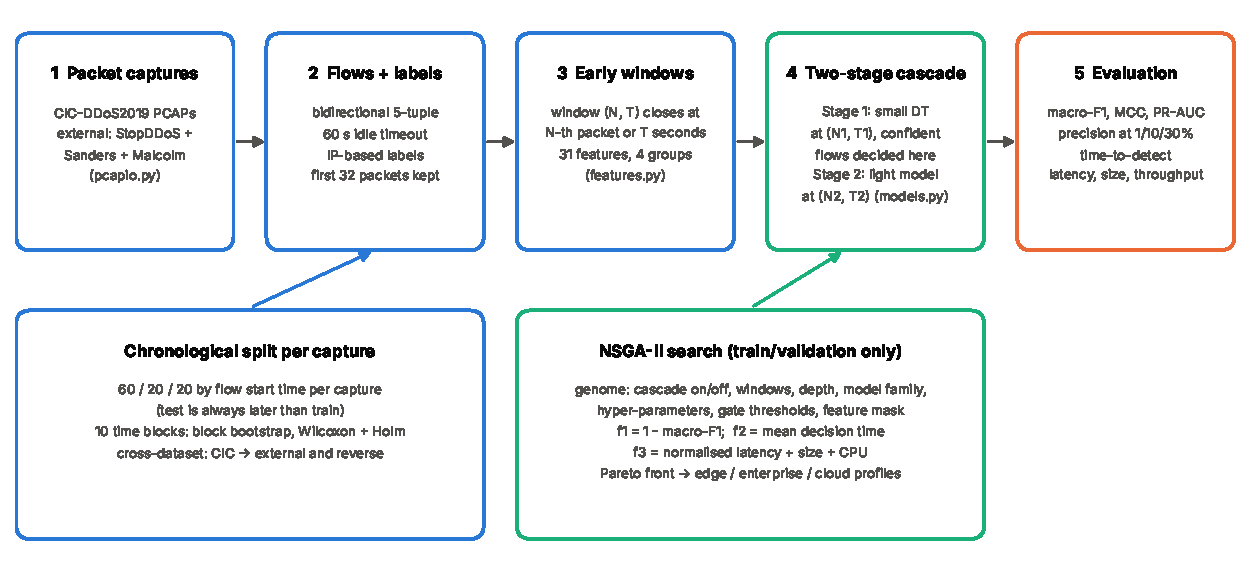
\includegraphics[width=\columnwidth]{fig0_architecture.pdf}
\caption{Implemented pipeline. The NSGA-II search sees only the training and validation split; the test split is used once.}
\label{fig:arch}
\end{figure}

\subsection{Early-window features}
The 31 features fall into four semantic groups following~\cite{elangovan2026}: \emph{intensity} (packet count, byte sum, mean, standard deviation, minimum and maximum packet length, byte and packet rates), \emph{temporal} (duration and inter-arrival-time statistics), \emph{direction} (fraction of packets and bytes from the initiator, responder packets, direction changes) and \emph{protocol} (protocol indicators, TCP flag fractions, mean window size, header lengths, fragment fraction, payload statistics). Each feature is tagged with the minimum number of packets it needs (e.g., inter-arrival times need two). IP addresses, ports, TTL and timestamps are never used as inputs.

\subsection{Confidence-gated cascade}
Stage~1 is a decision tree $h_1$ of depth $d_1$ applied at an early window $w_1=(N_1,T_1)$ on the features available at $N_1$ packets. Stage~2 is a lightweight model $h_2$ at a later window $w_2=(N_2,T_2)$ with $N_2>N_1$ and $T_2\ge T_1$. With gate thresholds $\tau_{lo}<\tau_{hi}$, the prediction and the decision time are given by Eqs.~\eqref{eq:cascade} and~\eqref{eq:cascadetime},
\begin{equation}
\hat{y}_f = \begin{cases} 1 & s_1 \ge \tau_{hi},\\ 0 & s_1 \le \tau_{lo},\\ \mathbf{1}[s_2\ge 0.5] & \text{otherwise,}\end{cases}
\label{eq:cascade}
\end{equation}
\begin{equation}
\tau(f) = \begin{cases} \tau_{w_1}(f) & s_1\notin(\tau_{lo},\tau_{hi}),\\ \max\big(\tau_{w_1}(f),\tau_{w_2}(f)\big) & \text{otherwise,}\end{cases}
\label{eq:cascadetime}
\end{equation}
where $s_k=h_k(\phi_{w_k}(f))$. Algorithm~\ref{alg:cascade} gives the inference procedure. Both stages are trained on the full training split with balanced class weights.

\begin{algorithm}[!t]
\caption{Cascade inference for one flow}\label{alg:cascade}
\begin{algorithmic}[1]
\Require packets of flow $f$; stages $(h_1,w_1)$, $(h_2,w_2)$; gate $\tau_{lo},\tau_{hi}$
\State buffer packets until window $w_1$ closes (Eq.~\ref{eq:tau})
\State $s_1 \gets h_1(\phi_{w_1}(f))$
\If{$s_1 \ge \tau_{hi}$} \Return attack at $\tau_{w_1}(f)$
\ElsIf{$s_1 \le \tau_{lo}$} \Return benign at $\tau_{w_1}(f)$
\EndIf
\State continue buffering until window $w_2$ closes
\State $s_2 \gets h_2(\phi_{w_2}(f))$
\State \Return $\mathbf{1}[s_2 \ge 0.5]$ at $\max(\tau_{w_1}(f),\tau_{w_2}(f))$
\end{algorithmic}
\end{algorithm}

\subsection{Multi-objective configuration search}
A configuration $\theta$ comprises: cascade on/off; $N_1\in\{1,2,3,4\}$; $T_1\in\{50,100,500\}$\,ms; $d_1\in\{2,\dots,5\}$; $N_2\in\{2,3,4,8,16,32\}$; $T_2\in\{50,100,500,2000\}$\,ms; a Stage-2 family (decision tree, RF, histogram gradient boosting, $k$NN, LR, multilayer perceptron) with one of four hyper-parameter settings; $\tau_{lo},\tau_{hi}$; and a 31-bit feature mask $\mathbf{m}$. A repair operator enforces $N_2>N_1$, $T_2\ge T_1$ and $\|\mathbf{m}\|_1\ge2$. On the validation split $\mathcal{V}$, three objectives are minimised:
\begin{align}
f_1(\theta) &= 1-\text{macro-}\fone(\theta;\mathcal{V}),\\
f_2(\theta) &= \frac{1}{|\mathcal{V}_1|}\sum_{f\in\mathcal{V}_1}\tau_\theta(f),\\
f_3(\theta) &= \tfrac13\Big(\tfrac{\ell_\theta}{\ell_{\mathrm{ref}}}+\tfrac{b_\theta}{b_{\mathrm{ref}}}+\tfrac{c_\theta}{c_{\mathrm{ref}}}\Big),
\end{align}
where $\mathcal{V}_1$ is the set of attack flows; $\ell$, $b$ and $c$ are single-flow latency, serialised model size and CPU time per flow (Stage-2 terms weighted by the deferral rate); and the reference is a 100-tree RF on all features at $N=32$, $T=2$\,s. NSGA-II~\cite{deb2002} uses non-dominated sorting, crowding distance, binary tournament selection, uniform crossover and per-gene mutation. Search quality is measured by the hypervolume of the front after normalising $(f_1/0.05,\,f_2/2\,\mathrm{s},\,f_3/3)$ with reference point $(1,1,1)$.

\subsection{Operating-point selection and changes after Phase~2}
Three deployment profiles are selected from the validation front: \emph{edge} (model $\le$64\,KB, $f_2\le$100\,ms, macro-$\fone\ge$0.995, minimum $f_3$), \emph{enterprise} (model $\le$1\,MB, macro-$\fone\ge$0.998, minimum $f_2$) and \emph{cloud} (maximum macro-$\fone$). The enterprise profile was fixed in advance as the main configuration. Relative to the Phase~2 plan, the implementation (i) uses raw CIC-DDoS2019 captures of both days instead of three datasets, (ii) replaces XGBoost with histogram gradient boosting and SHAP with permutation importance, (iii) replaces Raspberry~Pi measurements with a single-threaded CPU core, (iv) adds an Isolation Forest fallback as an extension, and (v) runs one search seed on the full data. \authornote{Authors: state the Phase~2 instructor feedback and how it was addressed here.}

% =====================================================================
\section{Experimental Setup}\label{sec:setup}
\subsection{Datasets and labelling}
\emph{CIC-DDoS2019}~\cite{sharafaldin2019} was captured on two days. The present study uses a selection of the 200\,MB capture files covering the start, middle and end of every attack and all benign-heavy periods, identified from capture timestamps and the share of attacker traffic in each file. A flow is labelled as an attack if one endpoint is the attacker host 172.16.0.5; its attack type is given by the capture file's position on the attack timeline, and two stretches of uncertain type were excluded. Because spoofed floods create a new flow for almost every packet, one in 20 attack flows was sampled by a stable hash of the flow key, and at most 1{,}000 attack and 5{,}000 benign flows were kept per file. The training day (1 Dec 2018) yields \RnTrain\ flows in 12 attack types (NTP, DNS, LDAP, MSSQL, NetBIOS, SNMP, SSDP, UDP, UDP-Lag, WebDDoS, SYN, TFTP) and \RnTrainBen\ benign flows. The test day (3 Nov 2018) yields \RnTest\ flows (\RnTestBen\ benign) in seven types, including PortMap, which never occurs in training.

The \emph{external set} comes from different networks: 21{,}794 attack flows from 18 real-world and laboratory DDoS captures~\cite{stopddos2022} and 7{,}323 benign flows from everyday traffic captures~\cite{sanders,malcolm}. It is used only for testing transfer, in both directions.

\subsection{Splits, baselines and metrics}
Training and validation use the first 80\% and last 20\% (by flow start time) of each training-day capture file; the whole test day is held out. Each test file is cut into ten contiguous time blocks, and block $j$ of every file is pooled into composite block $j$ for statistics.

The 16 baselines comprise: complete-flow RF (100 trees), gradient-boosted trees and MLP; the base method~\cite{ebrahem2026} re-implemented as CNB, $k$NN, RF and LR with NearMiss-1 under-sampling; Extra-Trees top-10 feature selection with RF, LR and Naive Bayes~\cite{nawaz2025}; one-class SVM and Isolation Forest trained on benign flows at $(N{=}8,T{=}0.5\,\mathrm{s})$~\cite{lamptey2025}; fixed early RF at $(8, 0.5\,\mathrm{s})$ and depth-8 tree at $(2, 0.1\,\mathrm{s})$; and the best configurations of random search and of a GA that optimises $f_1$ only, with the same budget as NSGA-II.

The metrics are macro-$\fone$, MCC, false-positive and false-negative rates, per-family recall, time-to-detect, and onset-to-first-alert per capture file. Precision at attack prevalence $\pi$ is obtained by re-weighting benign flows by $w_0 = n_1(1-\pi)/(\pi n_0)$, giving $\mathrm{Prec}_\pi = \mathrm{TP}/(\mathrm{TP}+w_0\mathrm{FP})$. Cost is measured as single-flow latency (feature extraction plus inference, p50/p95), batched throughput, model size and per-flow packet state. Uncertainty is reported as 95\% block-bootstrap confidence intervals (500 resamples). Paired Wilcoxon signed-rank tests on per-block macro-$\fone$ against the main configuration are Holm-corrected, with rank-biserial effect size $r$.

\subsection{Implementation details}
All components are implemented in Python with NumPy, SciPy and scikit-learn~\cite{sklearn2011}; no packet library is used. Models use balanced class weights; scalers are fitted inside each pipeline on training data. NSGA-II, random search and the GA each use a population of 32 for 24 generations (\Revals\ unique evaluations), seed~0; model seeds are 0. Experiments ran on the authors' Windows laptop; the cost benchmark used one thread (\texttt{OMP\_NUM\_THREADS=1}). A pilot on a 20{,}000-flow CIC-DDoS2019 sample with three search seeds preceded the full study.

% =====================================================================
\section{Results and Analysis}\label{sec:results}
\subsection{Selected configuration and overall results}
The enterprise configuration is a depth-\ReOneD\ decision tree at $N_1{=}\ReNone$, $T_1{=}\ReTone$\,ms, deferring flows with $s_1\in(\ReTlo,\ReThi)$ to a 50-tree RF at $N_2{=}\ReNtwo$, $T_2{=}\ReTtwo$\,ms, on \ReFeat\ features. Only \RmainDefer\ of flows reach Stage~2. Table~\ref{tab:main} reports the held-out results. The cascade reaches macro-$\fone$ \RmainFone\ [\RmainCIlo, \RmainCIhi] and MCC \RmainMCC, with FPR \RmainFPR\ and FNR \RmainFNR; it misses \Rmissed\ of \RnTestAtk\ attack flows. PortMap, absent from training, is detected at \RmainPortMap.

\begin{table*}[!t]
\centering
\caption{Results on the held-out test day (3 Nov 2018, \RnTest\ flows). TTD: median time-to-detect from a flow's first packet. Prec@1\%: precision at 1\% attack prevalence. Ext.: macro-$\fone$ on the external network after training on CIC. $p$: Holm-corrected Wilcoxon $p$ against the main configuration (10 blocks).}\label{tab:main}
\footnotesize
\begin{tabular}{lcccccccc}
\toprule
Detector & Macro-$\fone$ & 95\% CI & MCC & FPR (\%) & TTD & Prec@1\% & Ext. & $p$ \\
\midrule
Proposed cascade (enterprise) & 0.9987 & [0.998, 0.999] & 0.997 & 0.42 & 50\,ms & 0.708 & 0.631 & -- \\
Proposed (edge) & 0.9856 & [0.983, 0.989] & 0.972 & 4.75 & 100\,ms & 0.175 & 0.708 & 0.037 \\
Proposed (cloud) & 0.9971 & [0.997, 0.998] & 0.994 & 0.96 & 500\,ms & 0.513 & 0.484 & 0.037 \\
Fixed early DT-8 ($N{=}2$, 100\,ms) & 0.9985 & [0.998, 0.999] & 0.997 & 0.27 & $<$0.01\,ms & 0.791 & 0.508 & 0.322 \\
Fixed early RF-100 ($N{=}8$, 500\,ms) & 0.9970 & [0.996, 0.997] & 0.994 & 0.77 & 500\,ms & 0.567 & 0.591 & 0.037 \\
Full-flow RF-100 & 0.9957 & [0.994, 0.997] & 0.991 & 1.32 & 60.0\,s & 0.433 & 0.666 & 0.037 \\
Full-flow GBDT & 0.9978 & [0.997, 0.998] & 0.996 & 0.63 & 60.0\,s & 0.615 & 0.641 & 0.037 \\
Full-flow MLP & 0.9860 & [0.985, 0.987] & 0.972 & 3.54 & 60.0\,s & 0.222 & 0.269 & 0.037 \\
ET-top10 + RF~\cite{nawaz2025} & 0.9958 & [0.995, 0.996] & 0.992 & 1.14 & 60.0\,s & 0.470 & 0.724 & 0.037 \\
Isolation Forest~\cite{lamptey2025} & 0.9488 & [0.944, 0.953] & 0.902 & 15.86 & 500\,ms & 0.060 & 0.593 & 0.037 \\
One-class SVM~\cite{lamptey2025} & 0.7531 & [0.742, 0.763] & 0.576 & 6.59 & 500\,ms & 0.111 & 0.649 & 0.037 \\
Random-search best & 0.9962 & [0.996, 0.997] & 0.992 & 1.16 & 500\,ms & 0.465 & 0.604 & 0.037 \\
GA (F1 only) best & 0.9962 & [0.996, 0.997] & 0.992 & 1.27 & 500\,ms & 0.442 & 0.728 & 0.037 \\
\bottomrule

\end{tabular}
\end{table*}

All supervised detectors except the NearMiss variants exceed 0.98; they differ mainly in time and false positives. Complete-flow detectors decide at flow export, a median of \RrfTTDmed\,s, because UDP floods are never closed by FIN or RST; even if they could decide at the last packet, the median would be \RrfTTDend\,ms only because most reflection flows contain a single packet. The cascade is significantly more accurate than every baseline (Holm $p=0.037$, $r\ge0.96$) except the fixed depth-8 tree at two packets ($p=\RdtHolm$), which reaches \RdtFone\ with FPR \RdtFPR\ and decides at the second packet. The searched cascade therefore adds no measurable accuracy over a well-chosen fixed early tree on this data. The edge profile, selected on validation data, generalised worst to the test day (FPR \RedgeFPR), which shows the risk of choosing operating points on a single day's validation data.

\subsection{Accuracy and time against window size}
Fig.~\ref{fig:window} trains an RF at every window. One packet already yields macro-$\fone$ \RwinOne, and no larger window improves on it. From $N=3$ onwards, the many one- and two-packet reflection flows can only be decided when $T$ expires, so the mean decision time jumps from below 1\,ms to \RwinThreeA--\RwinThreeB\,s depending on $T$, while accuracy decreases slightly. This supports H1 for volumetric and reflection floods.

\begin{figure}[!t]
\centering
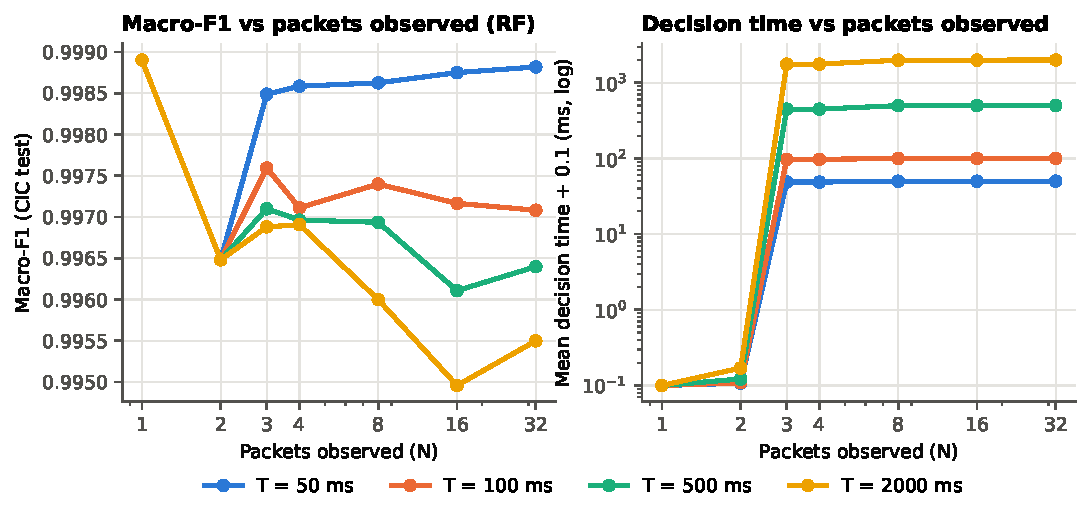
\includegraphics[width=\columnwidth]{fig1_window_sweep.pdf}
\caption{Macro-$\fone$ (left) and mean decision time of attack flows (right) for an RF trained at each window $(N,T)$; train 1 Dec, test 3 Nov.}
\label{fig:window}
\end{figure}

\subsection{Pareto front and search efficiency}
The validation front (Fig.~\ref{fig:pareto}) contains \RfrontN\ configurations, \RfrontTrees\ of which use a small decision tree (3--12\,KB) alone or as Stage~1, supporting H3. NSGA-II led in hypervolume for the first $\approx$450 evaluations, but the final values were \RhvN\ for NSGA-II, \RhvG\ for the F1-only GA and \RhvR\ for random search. With a single seed this comparison is not statistically meaningful; in the three-seed pilot NSGA-II exceeded random search on every seed (\RpilotHvN\ vs \RpilotHvR). Cheap and accurate trees are common in this search space, which limits the benefit of directed search.

\begin{figure}[!t]
\centering
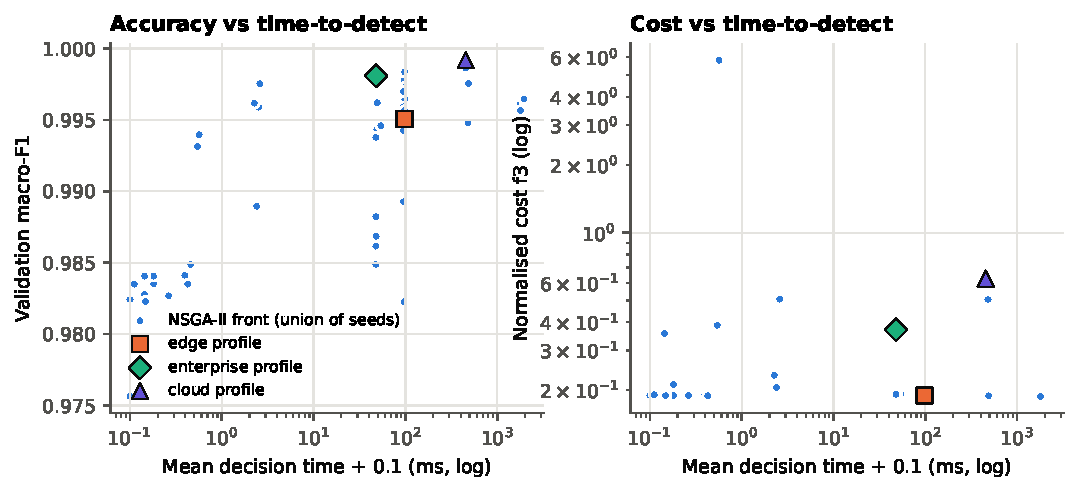
\includegraphics[width=\columnwidth]{fig3_pareto.pdf}
\caption{Validation Pareto front (NSGA-II, seed 0) with the edge, enterprise and cloud operating points.}
\label{fig:pareto}
\end{figure}

\subsection{Resource cost}
Table~\ref{tab:cost} and Fig.~\ref{fig:cost} report cost on one CPU core. The cascade's single-flow latency of \RmainLat\,ms is \RlatRatio$\times$ lower than the complete-flow RF (\RrfLat\,ms), and its throughput is \RmainThr\ versus \RrfThr\ flows/s, because the 50-tree Stage~2 runs for only \RmainDefer\ of flows. Latencies include Python per-call overhead; ratios rather than absolute values are the transferable result.

\begin{table}[!t]
\centering
\caption{Cost on one CPU core: single-flow latency (features + inference, ms), batched throughput (k flows/s), model size (KB) and packet state kept per open flow (bytes)}\label{tab:cost}
\footnotesize
\begin{tabular}{lccccc}
\toprule
Detector & p50 & p95 & kflows/s & KB & State \\
\midrule
Proposed (edge) & 0.55 & 0.74 & 107.7 & 4.6 & 2560 \\
Proposed (enterprise) & 0.58 & 1.10 & 85.9 & 312.1 & 320 \\
Proposed (cloud) & 3.00 & 3.69 & 91.4 & 134.1 & 320 \\
Fixed early DT-8 & 0.57 & 0.69 & 73.6 & 4.6 & 160 \\
Fixed early RF-100 & 9.41 & 13.72 & 31.2 & 544.3 & 640 \\
Full-flow RF-100 & 13.21 & 22.79 & 39.1 & 656.8 & flow \\
Full-flow GBDT & 7.15 & 27.55 & 22.1 & 596.9 & flow \\
$k$NN+NearMiss~\cite{ebrahem2026} & 2.62 & 6.39 & 10.5 & 1514.8 & flow \\
Isolation Forest & 10.52 & 18.24 & 39.4 & 924.3 & 640 \\
\bottomrule

\end{tabular}
\end{table}

\begin{figure}[!t]
\centering
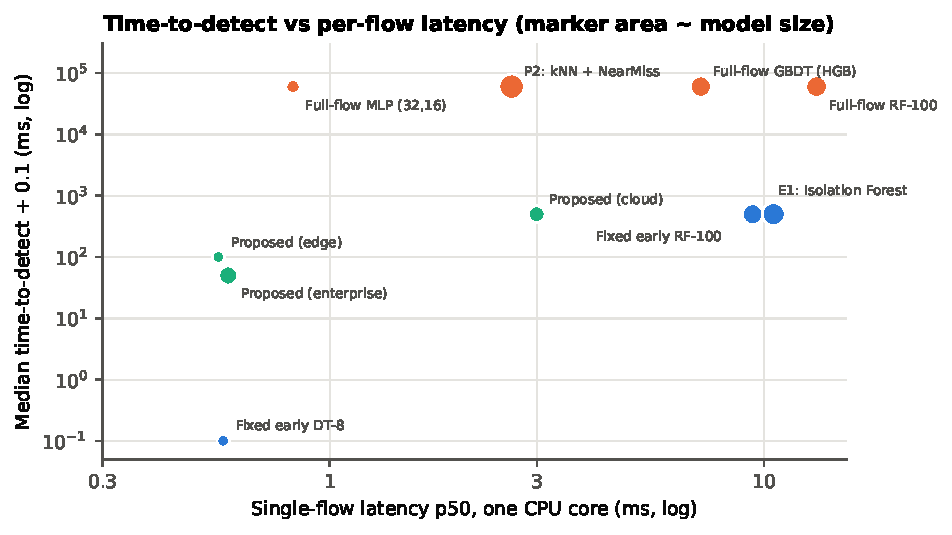
\includegraphics[width=\columnwidth]{fig6_time_cost.pdf}
\caption{Median time-to-detect against single-flow latency; marker area grows with model size. Early detectors (green, blue) lie four to six orders of magnitude below complete-flow detectors (orange).}
\label{fig:cost}
\end{figure}

\subsection{Realistic prevalence}
At 1\% attack prevalence (Fig.~\ref{fig:prev}), the expected precision is \RdtPone\ for the fixed tree, \RmainPone\ for the cascade, \RrfPone\ for the complete-flow RF and \RifPone\ for the Isolation Forest. Laboratory ratios (\RattackShare\ attacks on the test day) hide how strongly the false-positive rate governs operational usefulness.

\begin{figure}[!t]
\centering
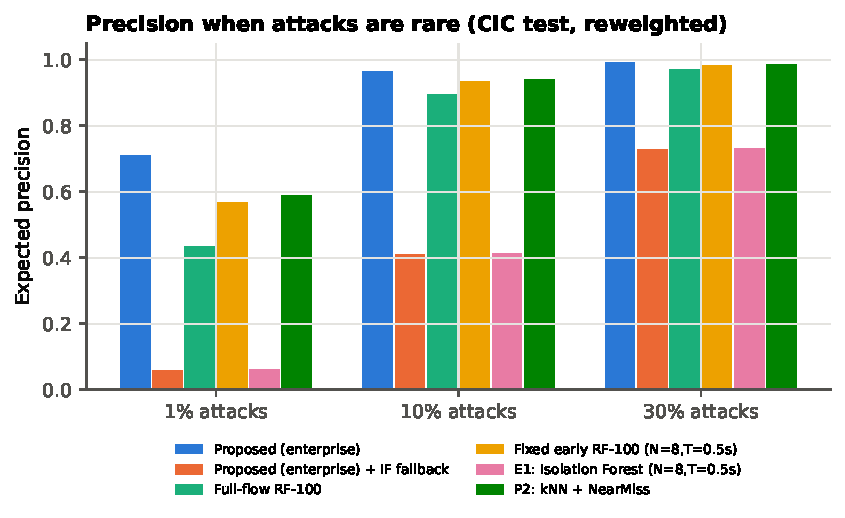
\includegraphics[width=\columnwidth]{fig7_prevalence.pdf}
\caption{Expected precision at 1\%, 10\% and 30\% attack prevalence (benign test flows re-weighted).}
\label{fig:prev}
\end{figure}

\subsection{Generalisation}
\emph{Across capture days and attack families}, the detectors generalise: when each of the \RloaoTypes\ shared families is removed from training in turn, the cascade still detects it with recall $\ge$\RloaoMin. \emph{Across networks}, transfer remains limited (Table~\ref{tab:transfer}). Trained on CIC, the cascade reaches \RmainExt\ on the external set, and the best detector reaches \RextBest. In the reverse direction, forests trained on the external set reach \RrevRF\ on CIC, whereas the cascade configuration chosen for CIC reaches \RrevMain. A configuration optimised on one network's validation data therefore carries that network's window and feature choices. Feature groups (Fig.~\ref{fig:groups}) do not support H2: direction features alone transfer best (\RdirExt) only by flagging \RdirFPR\ of external benign flows, temporal features alone transfer worst (\RtempExt), and removing them raises transfer to \RnoTempExt.

\begin{table}[!t]
\centering
\caption{Cross-network transfer (Ext: external set)}\label{tab:transfer}
\footnotesize
\begin{tabular}{llccc}
\toprule
Direction & Detector & Macro-$\fone$ & Recall & FPR (\%) \\
\midrule
CIC$\rightarrow$Ext & Proposed (enterprise) & 0.631 & 0.673 & 32.8 \\
CIC$\rightarrow$Ext & Proposed (edge) & 0.708 & 0.970 & 61.3 \\
CIC$\rightarrow$Ext & Fixed early DT-8 & 0.508 & 0.590 & 53.1 \\
CIC$\rightarrow$Ext & Full-flow RF-100 & 0.666 & 0.621 & 12.2 \\
CIC$\rightarrow$Ext & ET-top10 + RF & 0.724 & 0.705 & 11.6 \\
CIC$\rightarrow$Ext & GA (F1 only) best & 0.728 & 0.728 & 15.1 \\
Ext$\rightarrow$CIC & Proposed (enterprise) & 0.597 & 0.633 & 8.6 \\
Ext$\rightarrow$CIC & Full-flow RF-100 & 0.934 & 0.967 & 3.2 \\
Ext$\rightarrow$CIC & Fixed early RF-100 & 0.932 & 0.968 & 4.2 \\
\bottomrule

\end{tabular}
\end{table}

\begin{figure}[!t]
\centering
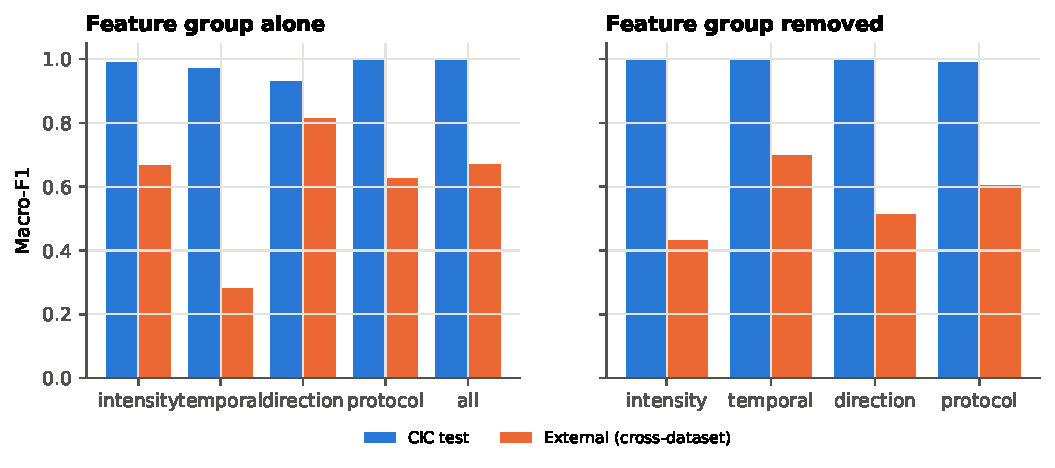
\includegraphics[width=\columnwidth]{fig9_group_transfer.pdf}
\caption{Macro-$\fone$ with each feature group alone (left) and removed (right), in-dataset and cross-network.}
\label{fig:groups}
\end{figure}

% =====================================================================
\section{Comparison with Base Papers}\label{sec:compare}
\subsection{Quantitative comparison}
Table~\ref{tab:p2} compares the proposed cascade with the base method of Ebrahem et al.~\cite{ebrahem2026}, re-implemented under the identical protocol (same flows, cross-day split, features and metrics). Absolute and relative improvements are computed as $\Delta = \fone^{\text{prop}}-\fone^{\text{base}}$ and $\Delta/\fone^{\text{base}}$. The best re-implemented base variant (\RbestPtwoName+NearMiss) reaches \RbestPtwo; the cascade improves on it by \RimpAbs\ (\RimpRel). It also decides at a median of \RmainTTDmed\,ms instead of 60\,s and is \RknnSpeed$\times$ faster per flow than the $k$NN variant (\RknnLat\,ms, \RknnSize\,KB). Table~\ref{tab:reported} lists the numbers reported in the base papers, which come from different data and splits and are therefore not directly comparable.

\begin{table*}[!t]
\centering
\caption{Quantitative comparison with the re-implemented base method ($^\dagger$ = re-implemented here under the identical protocol). Latency: single-flow p50 (ms). Improvement: absolute and relative macro-$\fone$ gain of the proposed cascade over each row.}\label{tab:p2}
\footnotesize
\begin{tabular}{lccccccc}
\toprule
Method & Macro-$\fone$ & FPR (\%) & FNR (\%) & Median TTD & Latency & KB & Improvement \\
\midrule
Ebrahem~\cite{ebrahem2026} CNB+NearMiss$^\dagger$ & 0.8728 & 13.62 & 5.72 & 60.0\,s & 0.89 & 3 & +0.1258 (+14.4\%) \\
Ebrahem~\cite{ebrahem2026} $k$NN+NearMiss$^\dagger$ & 0.7395 & 0.55 & 22.28 & 60.0\,s & 2.62 & 1515 & +0.2591 (+35.0\%) \\
Ebrahem~\cite{ebrahem2026} RF+NearMiss$^\dagger$ & 0.7523 & 0.51 & 20.81 & 60.0\,s & 9.18 & 151 & +0.2464 (+32.7\%) \\
Ebrahem~\cite{ebrahem2026} LR+NearMiss$^\dagger$ & 0.7979 & 0.64 & 15.82 & 60.0\,s & 0.79 & 2 & +0.2007 (+25.2\%) \\
Full-flow RF, class weights$^\dagger$ & 0.9957 & 1.32 & 0.02 & 60.0\,s & 13.21 & 657 & +0.0030 (+0.3\%) \\
\textbf{Proposed cascade} & 0.9987 & 0.42 & 0.01 & 50\,ms & 0.58 & 312 & -- \\
\bottomrule

\end{tabular}
\end{table*}

\begin{table}[!t]
\centering
\caption{Results reported in the base papers ($^*$ = taken from the original paper; different data and splits)}\label{tab:reported}
\footnotesize
\setlength{\tabcolsep}{3pt}
\begin{tabular}{L{1.9cm}L{2.7cm}L{3.0cm}}
\toprule
Paper & Reported$^*$ & This work \\
\midrule
Ebrahem~\cite{ebrahem2026} & Acc./$\fone$ $>$98\%, random split & \RmainFone\ macro-$\fone$, cross-day \\
Alabri~\cite{alabri2026} & 98.2\% acc.; 97.2\% external (CIC family) & \RmainFone\ cross-day; \RmainExt\ cross-network \\
Bocu~\cite{bocu2026} & 99.82\% acc.; 0.57\,s with 20 nodes & median TTD \RmainTTDmed\,ms on one core \\
\bottomrule
\end{tabular}
\end{table}

\subsection{Methodological comparison and source of the gain}
The cascade differs from the base method in three ways. (i) It decides from early windows instead of complete flows, which removes the flow-export delay entirely. (ii) It uses class weights instead of NearMiss-1. The ablation in Section~\ref{sec:ablation} shows that NearMiss alone causes most of the gap: with an identical RF and features, NearMiss gives \RbalNM\ and class weights \RbalCW. NearMiss-1 keeps the attack flows closest to benign ones, so the classifier learns a boundary that lets SYN and UDP-Lag floods pass (recall \RknnSynRec\ and \RknnLagRec\ for $k$NN). (iii) It gates a heavier model behind a small tree, which keeps the latency of a tree with the accuracy of a forest.

\subsection{Fairness and limitations of the comparison}
The base method was re-implemented on raw-capture flows with the present feature set rather than CICFlowMeter features, and on a cross-day rather than random split, so the re-implemented numbers are lower than those originally reported; the comparison is fair with respect to the present protocol only. Alabri et al.~\cite{alabri2026} and Bocu and Iavich~\cite{bocu2026} were not re-implemented because their pipelines or data are not public; their numbers are reported for context only. On the external network, the cascade (\RmainExt) is below the external accuracy reported by Alabri et al.\ (97.2\%), but that external set came from the same CIC family; on comparable data, the complete-flow RF also reaches only \RrfExt.

% =====================================================================
\section{Ablation Study}\label{sec:ablation}
Table~\ref{tab:ablation} and Fig.~\ref{fig:ablation} vary one component of the main configuration at a time.

\begin{table*}[!t]
\centering
\caption{Ablation of the main configuration (test day; Ext.: external macro-$\fone$; TTD: mean, ms; Lat.: single-flow latency, ms)}\label{tab:ablation}
\footnotesize
\begin{tabular}{lcccccc}
\toprule
Variant & Macro-$\fone$ & FPR\% & TTD & Ext. & KB & Lat. \\
\midrule
Full cascade (validation-selected) & 0.9987 & 0.42 & 49 & 0.631 & 312.1 & 0.63 \\
Stage 2 only & 0.9984 & 0.45 & 97 & 0.699 & 308.6 & 6.65 \\
Stage 1 only & 0.9974 & 0.11 & 49 & 0.658 & 312.1 & 0.59 \\
Stage 1 at $N_1{=}1$ & 0.9990 & 0.29 & $<$0.01 & 0.694 & 311.9 & 0.56 \\
Looser gate (0.30/0.60) & 0.9996 & 0.11 & 49 & 0.658 & 312.1 & 0.56 \\
Stage 2 at $T_2{=}50$\,ms & 0.9995 & 0.13 & 49 & 0.647 & 303.3 & 0.69 \\
All 31 features & 0.9971 & 0.71 & 49 & 0.451 & 368.3 & 0.61 \\
$-$ intensity & 0.9760 & 7.90 & 49 & 0.666 & 246.8 & 0.71 \\
$-$ temporal & 0.9943 & 1.67 & 49 & 0.753 & 321.9 & 0.64 \\
$-$ protocol & 0.9944 & 1.64 & 49 & 0.624 & 350.5 & 0.63 \\
$-$ direction & 0.9987 & 0.41 & 49 & 0.637 & 327.7 & 0.79 \\
Stage 2 = tree & 0.9967 & 1.10 & 49 & 0.609 & 8.0 & 0.59 \\
Stage 2 = LR & 0.9951 & 0.89 & 49 & 0.668 & 4.8 & 0.56 \\
Stage 2 = $k$NN & 0.9983 & 0.54 & 49 & 0.661 & 8726.0 & 0.60 \\
\bottomrule

\end{tabular}
\end{table*}

\begin{figure}[!t]
\centering
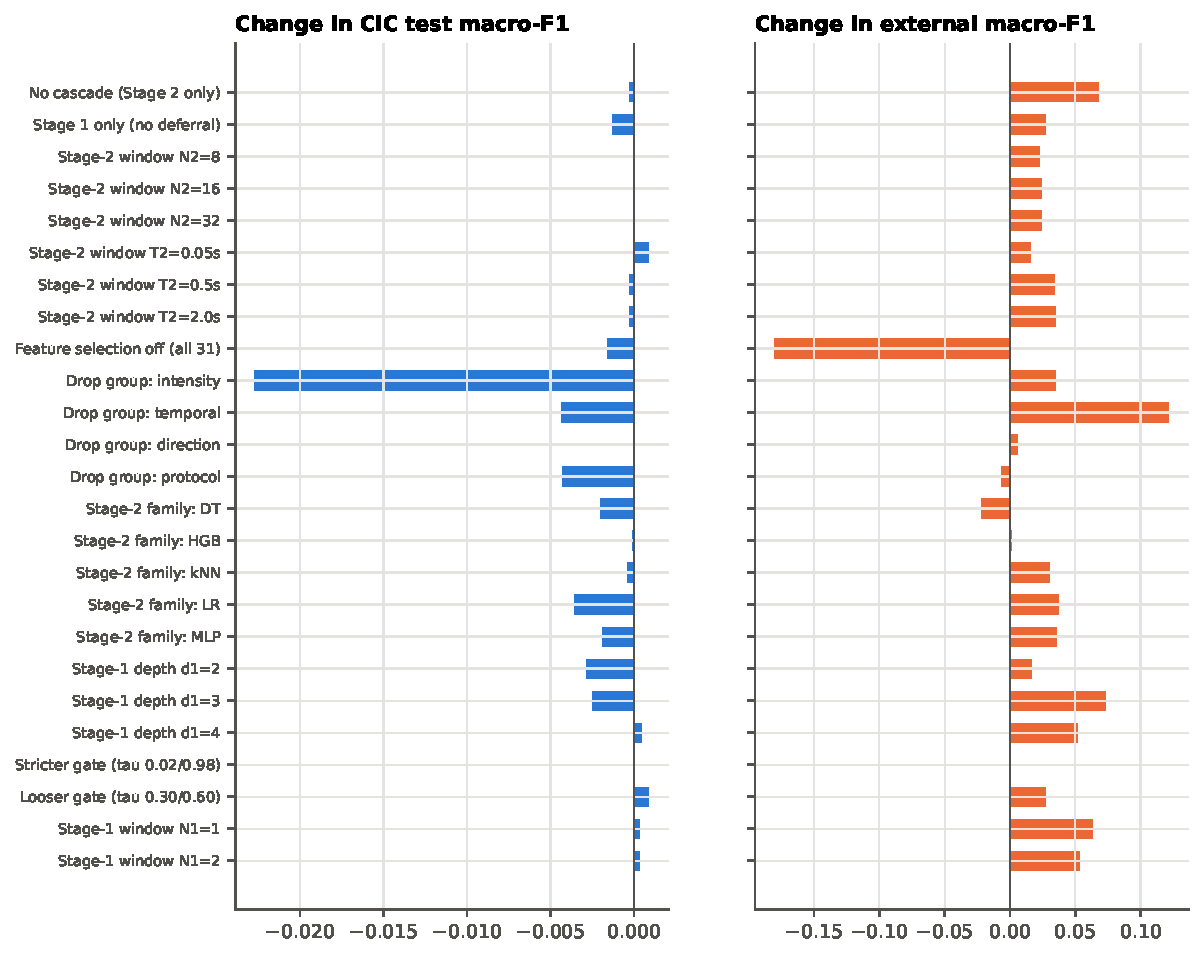
\includegraphics[width=\columnwidth]{fig10_ablation.pdf}
\caption{Change in macro-$\fone$ relative to the full configuration on the test day (left) and the external network (right).}
\label{fig:ablation}
\end{figure}

\emph{Cascade.} Stage~2 alone matches the cascade's accuracy (\RabSTwoF) but doubles the mean decision time (\RabSTwoTTD\ vs \RabFullTTD\,ms) and raises latency from \RabFullLat\ to \RabSTwoLat\,ms. Stage~1 alone is cheaper but less accurate (\RabSOneF). The gate therefore delivers forest accuracy at tree cost.
\emph{Windows and gate.} Moving Stage~1 to the first packet yields \RabNoneF\ with near-zero decision time, better than the validation-selected setting, which confirms that single-day validation does not identify the best test-day configuration.
\emph{Features.} Removing intensity features causes the largest loss (\RabIntF, FPR \RabIntFPR). Removing temporal features slightly reduces in-dataset accuracy but raises external macro-$\fone$ to \RabTempExt, and using all 31 features lowers it to \RabAllExt; feature selection on CIC validation data thus specialises the detector to CIC.
\emph{Model family.} Replacing the Stage-2 forest with a tree, LR or $k$NN changes in-dataset macro-$\fone$ by at most 0.004, while $k$NN needs an 8.7\,MB model.

% =====================================================================
\section{Discussion}\label{sec:discussion}
\subsection{Why the method works}
Permutation importance (Fig.~\ref{fig:imp}) shows that mean packet length and the variability of inter-arrival times carry nearly all of Stage~2's decisions on both the CIC test day and the external network (rank correlation \Rspear; \RpilotSpear\ in the pilot). Packet size is largely a property of the reflected service (large DNS, LDAP or NTP responses), which is visible in the first packet and explains why one or two packets suffice and why detection transfers across days. The same property explains the failure cases.

\begin{figure}[!t]
\centering
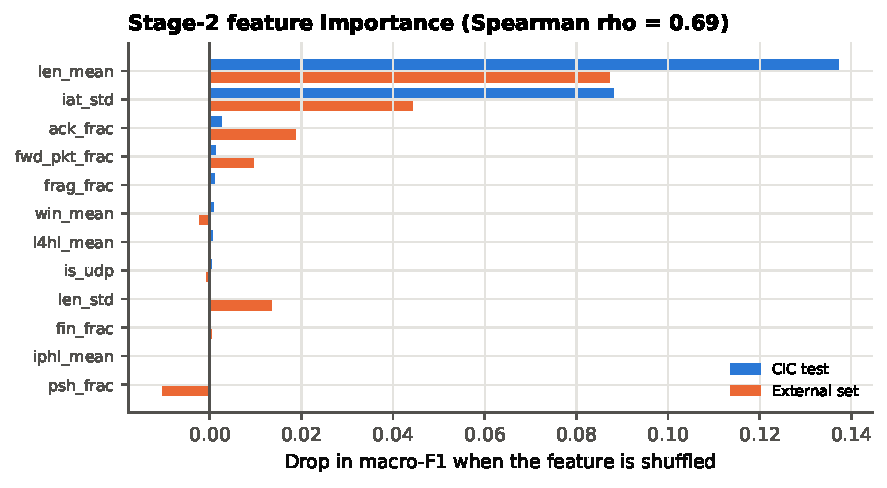
\includegraphics[width=\columnwidth]{fig12_importance.pdf}
\caption{Permutation importance of the Stage-2 features on the CIC test day and on the external network.}
\label{fig:imp}
\end{figure}

\subsection{Failure cases}
On the external network (Fig.~\ref{fig:ext}), false alarms concentrate on benign DNS (\RdnsFP), SIP, HTTP, Syslog and SSH traffic, whose first packets resemble reflection responses. Attacks with small or unusual packets---SYN-ACK reflection, SNMP and DNS-ANY amplification, random-protocol floods---are mostly missed. A slow-ramp stress test that stretches attack inter-arrival times by up to 50$\times$ leaves the cascade's recall at \RstressMain\ (the 8-packet RF drops to \RstressRF\ at 10$\times$), but an adaptive attacker that also changes packet sizes was not evaluated.

\begin{figure}[!t]
\centering
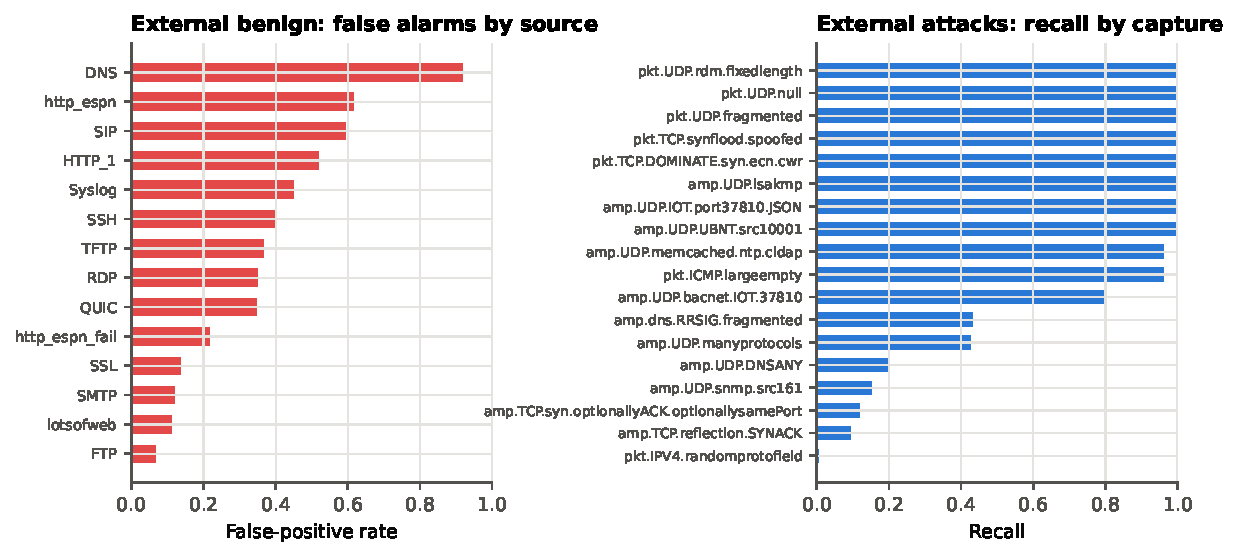
\includegraphics[width=\columnwidth]{fig13_external_errors.pdf}
\caption{External network: false-positive rate per benign source (left) and recall per attack capture (right).}
\label{fig:ext}
\end{figure}

\subsection{Practical implications}
Early windows remove the flow-export delay, which dominates time-to-detect, at no loss of accuracy within a network. A two-stage gate allows a gateway to process most flows with a tree of a few kilobytes. At realistic prevalence the false-positive rate, not macro-$\fone$, determines alert quality, so operating points should be chosen on precision at the expected prevalence.

\subsection{Pilot versus full data}
Moving from the 20{,}000-flow pilot to the full captures changed three conclusions: unseen SYN floods went from \RpilotSyn\ to \RmainSyn\ recall in leave-one-out tests, cross-network macro-$\fone$ of the cascade rose from \RpilotExt\ to \RmainExt, and feature importance became consistent across networks. Attack diversity in training matters more than model choice.

\subsection{Achievement of objectives}
Gap~1 (joint measurement of accuracy, delay and cost) is addressed for \RnDetectors\ detectors. Gap~3 (explicit trade-off optimisation) is addressed methodologically through a Pareto front and profile selection, but the data do not show the search outperforming a simple fixed tree or random search. Gap~2 (generalisation) is closed across capture days and to unseen families within CIC-DDoS2019, but not across networks.

\subsection{Threats to validity}
\emph{Internal:} attack types come from the capture timeline, and attack flows were sampled; one search seed was run; statistical tests use contiguous time blocks rather than independent sessions. \emph{External:} a single benchmark testbed was used for training; the external set combines attack and benign traffic from different sources, so part of its separability may reflect capture differences; no true low-rate attack data were available. \emph{Construct:} costs were measured in Python on a laptop core rather than on embedded hardware.

% =====================================================================
\section{Conclusion and Future Work}\label{sec:conclusion}
This paper presented an early-window, confidence-gated cascade for DDoS detection whose configuration is selected by multi-objective search over accuracy, time-to-detect and cost. On raw CIC-DDoS2019 captures with a cross-day split, it matched or exceeded complete-flow detectors in accuracy (macro-$\fone$ \RmainFone), decided within \RmainTTDmed\,ms instead of \RrfTTDmed\,s, and cost \RlatRatio$\times$ less per flow. It improved on the re-implemented base method by \RimpAbs\ macro-$\fone$. A fixed two-packet tree performed equally well, and transfer to an independent network remained limited. Future work will add a cross-network or unseen-family objective to the search, evaluate on true low-rate and adaptive attacks, and port the detector to programmable data planes or embedded hardware.

% =====================================================================
\section*{Declarations}
\noindent\textbf{Data and code availability.} CIC-DDoS2019 is available from the Canadian Institute for Cybersecurity; the external captures are public~\cite{stopddos2022,sanders,malcolm}. The code, the capture-file selection, all evaluated search configurations and result files are provided with this submission. \authornote{Authors: add the repository link.}

\noindent\textbf{Conflict of interest.} The authors declare no conflict of interest.

\noindent\textbf{Funding.} This research received no external funding.

\noindent\textbf{Use of AI tools.} Generative AI tools (Claude, Anthropic) were used to assist with code development, data-processing scripts and language editing of this manuscript. All reported results were produced by executing the released code on the stated data. The authors reviewed all content and take full responsibility for it. \authornote{Authors: adjust to reflect your actual use.}

\section*{Acknowledgements}
The authors thank the course instructors for their guidance.

\bibliographystyle{IEEEtran-doi}
\bibliography{references}

\end{document}
